% this file is called up by thesis.tex
% content in this file will be fed into the main document

%: ----------------------- name of chapter  -------------------------
\chapter{Existence and Connectedness Theorems} % top level followed by section, subsection


%: ----------------------- paths to graphics ------------------------

% change according to folder and file names
\ifpdf
    \graphicspath{{figures/}{figures/}{figures/}}
\else
    \graphicspath{{figures/}{figures/}}
\fi

%: ----------------------- contents from here ------------------------


The scope of this Chapter is to achieve a generalization of two basic results of the classical \BN Theory, the Existence and Connectedness Theorems, to the case of an arbitrary algebraically closed field. The content of the Theorems underlines the crucial role of the \BN number $\rho$ in the study of linear series: in fact, a non negative value of $\rho$ implies that $\Wdr$ is not empty and, moreover, $\rho>0$ ensures its connectedness.
These results were proved in the last decades for curves over the complex numbers but, as we will see, can be extended to closed fields of positive characteristic.\\
Thanks to a general result on degeneracy loci proved by Fulton -- Theorem \ref{theo:alg} of Appendix A -- the Existence and Connectedness Theorems will follow immediately, but first we need to show that Fulton's hypothesis are met in our situation. The first step is to show that $\Wdr$ can be seen as a degeneracy locus of a morphism of vector bundles
$$ \ph: E\tolong F $$
where $E$ and $F$ arise from a specific cohomology sequence associated to the universal line bundle $\scL$. It is crucial to choose these vector bundles in a smart way, in order to simplify the following and last step, in which we need to show that the tensor product $E^*\otimes F \cong \Hom(E,F)$ is an ample vector bundle.

\section{An alternative perspective on $\Wdr$}\label{sec:alternative}

	\begin{notation}
		For every natural number $d\in \N$, let $M=\sum_{i=1}^m p_i$ be a divisor of high degree $m\geq2g-d$ on $X$ and set $n:=m+d$.
	\end{notation}	
	
	To begin, we will give a recipe to construct an explicit universal line bundle $\scL_n$ of degree $n$ which enjoys the characterizing universal property. Because of the uniqueness up to isomorphisms of such an universal object, the explicit recipe given in  this Section is compatible with the non-constructive approach we adopted in the previous Chapters.

	For now and for the rest of the section, choose a closed point $Q\in X$ and define 
	$$ [Q] := \set{ D\in \Dn \mid Q \in \Supp(D) } \subset \Dn $$
	Further, let $\Delta$ be a universal divisor of degree $n$, let $u:\Dn\to\Pn$ the \AJJ map and $\pi:Z=X\times\Dn\to\Dn$ the natural projection. 
	\begin{defi}\label{def:universal_lb}
		We define a universal line bundle $\scL_n \to X\times\Pn$ of degree $n$ by
		$$ \scL_n := (1_X\times u)_*(\calO_Z(\Delta - \pi^* [Q])) $$
	\end{defi}
	Notice that the above pushforward gives in fact a line bundle, the reason being that the \AJJ map $u$ is onto $\Pn$ since $n$ is greater than $2g-1$.
	Moreover, it is easy to check that the resulting line bundle enjoys the universal property of a universal line bundle, but we leave the details to the interested reader. \\

	Recall that the moduli variety $\Wdr$ was defined as a Fitting scheme associated to the sheaf $R^1\nu_{*}\scL_d$, where $\scL_d$ is a universal line bundle of degree $d$. 
	It will be convenient, in this section, to \emph{translate} our point of view and work directly in higher degree. 
	Hence, using the recipe provided by Definition \ref{def:universal_lb}, choose $\scL_n$ to be a universal line bundle of degree $n=d+m$. 
	Further, let $\Gamma = M\times \Pn$ and use the isomorphism
	$$ a:\Pd\toiso\Pn, \qquad L\mapsto L\otimes \calO(M) $$
	to define the universal line bundle $\scL_d$ of degree $d$ as the pull-back of $\scL_n(-\Gamma)$ 
	$$ \scL_d := a^*\scL_n(-\Gamma). $$
	We claim that the image $a(\Wdr)\subset \Pn$ is the closed subscheme $Y$ corresponding to the Fitting ideal $\Fitt_{t}(R^1\nu_{*}\scL_n(-\Gamma)) $ with $t=g-d+r-1$, the reason being that the scheme theoretic preimage $a^{-1}(Y)$ corresponds to the ideal sheaf
	$$ 	a^*\Fitt_{t}(R^1\nu_{*}\scL_n(-\Gamma)) 
	= 	\Fitt_{t}(a^*R^1\nu_{*}\scL_n(-\Gamma)) 
	= 	\Fitt_{t}(R^1\nu_{*} \scL_d)
	$$
	as one sees invoking Corollary \ref{coro:functoriality} and recalling that Fitting ideals -- defined through a free presentation -- are not affected by tensor product.
	Therefore we understand that $\Wdr$ can also be seen as the $(m-g+d-r)$-degeneracy locus of the evaluation map
	$$ E:=\nu_{*} \scL_n \;\longrightarrow\; \nu_{*} (\scL_n / \scL_n(-\Gamma))=:F, $$
	which will turn out to be a convenient point of view, as we will see in the next Section.


\section{Ampleness of $(\nu_{*} \scL)^* \otimes \nu_{*} (\scL/\scL(-\Gamma))$}\label{sec:ampleness}

	We start by exploiting the choice of the vector bundle $F = \nu_{*} (\scL_n / \scL_n(-\Gamma))$, showing that it admits a simple description in the following Lemma. 

	\begin{notation}
		For the rest of this Section we will write $\scL=\scL_n$ to denote the universal line bundle of degree $n$. Further, for any closed point $P\in X$, denote by $\Gamma_P $ the divisor $P \times \Pn \subset X\times \Pn$.
	\end{notation}
	\begin{defi}\label{def:alg_equiv}
		Two line bundles $L_1$ and $L_2$ over a scheme $Y$ are said to be \textbf{algebraically equivalent} if there exist a connected scheme $T$, two closed points $t_1,t_2\in T$ and a line bundle $L$ over $Y\times T$ such that
		$$ L_{\mid Y\times t_1} \cong L_1 \AND L_{\mid Y\times t_2} \cong L_2. $$
	\end{defi}

	\begin{lemm}\label{lemm:alg_trivial}
		If the divisor $M=\sum_{i=1}^m p_i$ is reduced, then $F=\nu_{*} (\scL / \scL(-\Gamma))$ is a direct sum of algebraically trivial line bundles.
	\end{lemm}
	\begin{proof}
		Let $P$ be a closed point of $X$ and notice that $\scL/\scL(-\Gamma_P)$ is just the restriction of $\scL$ to $\Gamma_P$. Therefore, from the natural isomorphism
		$$ \calO_{X\times X_n}(\Delta)\otimes \calO_{\{P\}\times X_n} \cong \calO_{X_n}([P]) $$
		together with the explicit form of the universal line bundle $\scL = (1_X\times u)_*(\calO(\Delta - \pi^* [Q]))$, we deduce that 
		\begin{equation}\label{eq:description}
			\nu_{*} \left(\scL/\scL(-\Gamma_P)\right) \cong u_* \calO_{X_n}([P]-[Q]).
		\end{equation}
		To show that $\nobreak{u_* \calO_{X_n}([P]-[Q])}$ is algebraically equivalent to the trivial bundle, following the notation of Definition \ref{def:alg_equiv} we can take $L=\scL$, $T=X$ and $t_1=P$, $t_2=Q$ for the points. Indeed one can easily see that we have
		$$ \scL_{\mid \Pn\times \{P\}} \cong u_* \calO_{X_n}([P]-[Q]) \AND \scL_{\mid \Pn\times \{Q\}} \cong u_*\calO_{X_n} \cong \calO_{\Pn} $$
	\end{proof}
	\begin{rema}
		In the case of a non-reduced $M$ (i.e.\ if the $p_i$'s are not distinct), the statement of the above Lemma is no longer true. However, one can still show that $F$ admits a filtration with successive quotients being trivial line bundles. The latter fact is enough for the next arguments, allowing minor modifications. Nevertheless, we will just deal with the reduced case here, leaving the generalisation as an exercise for the reader.
	\end{rema}

	Our next objective is to show that the vector bundle $\nu_{*} \scL$ is ample, but first of all we need to clarify what ampleness means in this setting.
	\begin{defi}
		A vector bundle $E$ over a variety $X$ is said to be \textbf{ample} if the tautological line bundle $\calO_{\PP E^*}(1)$ is ample.
		\begin{comment}
			\item The tautological line bundle $\calO_{\PP E^*}(1)$ of $\PP E^*$ is ample
			\item For every coherent sheaf $\scr{F}$ over $X$ there exists $n_0\in \N$ such that
			$$ H^i(X, \scr{F}\otimes \Sym^n E) = 0 \qquad \forall n\geq n_0, \quad \forall i > 0 $$ 
		\end{comment}
	\end{defi}

	We now move to the vector bundle $E=\nu_{*} \scL$, looking in particular to its associated projectified bundle.
	\begin{prop}
		The projectified bundle $\PP E$ is naturally isomorphic to $X_n$ and the projection $\PP E \to \Pn$ coincides with the Abel-Jacobi map $X_n \overset{u}\longrightarrow \Pn$. Moreover, under this isomorphism we have
		$$ \calO_{\PP E}(1) \cong \calO_{X_n}([Q]) $$
	\end{prop}
	\begin{proof}
		Every fiber of $E=\nu_{*}\scL$ over $L\in \Pn$ coincides with the vector space of global sections $H^0(X,L)$, hence the points of $\PP E$ are pairs $(L,\sigma)$ where $\sigma$ is a $1$-dimensional subspace of $H^0(X,L)$, which is the same as a divisor $D\in |L|$. Therefore $\PP E \cong X_n$, and the projection onto $\Pn$ is given by the Abel-Jacobi map $(L,\sigma) \mapsto L$.\\

		For the second statement, consider the natural map
		$$ \psi: E \to \nu_*(\scL/\scL(-\Gamma_Q)) $$
		obtained by evaluation and restriction, an pull it back via $u$ to get a morphism
		$$ \calO_{\PP E}(-1)\to u^* E \to u^*(\nu_*(\scL/\scL(-\Gamma_Q))) $$
		where the last bundle is trivial, as one immediately sees from the description \ref{eq:description} given in the proof of Lemma \ref{lemm:alg_trivial}. Hence passing to the dual we find the transpose morphism
		$$ \calO_{X_n} \to \calO_{\PP E}(1) $$
		which, by definition of $\psi$, vanishes of order $1$ over $[Q]$. Therefore we obtain an induced isomorphism
		$$\calO_{X_n}([Q]) \toiso \calO_{\PP E}(1)$$ 
	\end{proof}
	Exploiting the description of $\calO_{\PP E}(1)$ we just achieved, we will now show that $E^*$ is ample.
	\begin{prop}
		The vector bundle $E^* = (\nu_{*}\scL)^*$ is ample.
	\end{prop}
	\begin{proof}
		Our objective is to show that $\calO_{\PP E}(1)\cong \calO_{X_n}([Q])$ is ample as a line bundle over $X_n$, so it is useful to apply Proposition \ref{prop:Nakai} of Appendix A to the quotient map $\zeta:X^n\to X_n$ and look at the pullback of $\calO_{X_n}([Q])$. This can be written as
		$$ \zeta^* \calO_{X_n}([Q]) = \bigotimes_{i=1}^n \pi_i^* \OX(Q)\,, $$
		where $\pi_i:X^n\to X$ is the projection on the $i$-th component.\\
		Now notice that $\OX(Q)$ is ample being of positive degree and, so, from Lemma \ref{lemm:tensor_ampleness} of Appendix A it follows that the tensor product $\otimes_{i=1}^n \pi_i^* \OX(Q)$ is ample as well, showing that $\zeta^* \calO_{X_n}([Q])$ and hence $\calO_{X_n}([Q])$ is ample, as desired.
	\end{proof}
	Now, since we showed that $E^*$ is ample and $F$ is the direct sum of algebraically trivial line bundles, it follows immediately that the vector bundle
	$$ E^*\otimes F \cong \operatorname{Hom}(E,F) $$
	is ample. This is exactly what we need, in the following section, to apply Theorem \ref{theo:alg} of Appendix A to our situation thus getting the Existence and Connectedness Theorems.

\section{Existence and Connectedness Theorems}
	In the previous section we proved the ampleness of the vector bundle 
	$$ E^*\otimes F = (\nu_{*} \scL)^* \otimes \nu_{*} (\scL/\scL(-\Gamma)) $$
	and, as a consequence, we can apply Theorem \ref{theo:alg} of Appendix A to the bundle morphism
	$$ \nu_{*} \scL \;\overset{\ph}\longrightarrow\; \nu_{*} (\scL / \scL(-\Gamma)) $$
	getting as a result the Existence and Connectedness Theorems.
	\begin{namedtheo}[Existence Theorem]\label{thm:existence}
		Let $X$ be a smooth projective curve of genus $g$ and $d,r\in \N$ such that
		$$ \rho = g-(r+1)(g-d+r) \geq 0. $$
		Then the moduli variety $\Wdr$ is not empty.
	\end{namedtheo}
	\begin{namedtheo}[Connectedness Theorem]
		Let $X$ be a smooth projective curve of genus $g$ and $d,r\in \N$ such that
		$$ \rho = g-(r+1)(g-d+r) > 0. $$
		Then the moduli variety $\Wdr$ is connected.	
	\end{namedtheo}
	\begin{proof}
		Since pullback preserves the rank of vector bundles, we deduce from Remark \ref{rema:ranks} that $E$ and $F$ have ranks $e=d+m-g+1$ and $f=m$.
		Then, recall from the last Section that $\Wdr$ can be interpreted as the degeneracy locus
		$$ \Wdr = \FittS_{(s-1)}(R^1\nu_{*}\scL(-\Gamma)) = D_{(m-s)}(\ph) $$
		with $s=g-d+r$. Further, we know that the dimension of $Y=\Pn$ is given by $g$, so a trivial computation shows that
		$$ \dim(Y) \geq (e-(m-s))(f-(m-s)) \iff g \geq (r+1)(g-d+r) \iff \rho \geq 0\,, $$
		therefore both the Existence and Connectedness Theorems follow immediately from Theorem \ref{theo:alg} of Appendix A.
	\end{proof}
	%
	Looking at the above results, a natural question to ask is whether a negative value of the \BN number $\rho$, for given integers $d$ and $r$, implies the absence of $g_d^r$ on the curve $X$. This question admits a positive answer in the classical setting of a smooth projective curve over $\C$, as the following Theorem -- originally stated by Brill and Noether and then proved by Griffiths and Harris -- implies.
	\begin{namedtheo}[Dimension Theorem]
		Let $X$ be a smooth projective curve of genus $g$ over the complex numbers and fix integers $d\geq 1$ and $r\geq 0$. Then the variety $\Gdr$ is empty if $\rho<0$, while it is reduced of pure dimension $\rho$ if $\rho\geq 0$.
	\end{namedtheo}
	The Dimension Theorem was out of the scope of this thesis, nevertheless our intuition suggests that such a result should remain valid over a more general algebraically closed field $k$. In any case we would like to highlight the fact that the Dimension Theorem allows to further restrict the region of special exceptional divisors, thus obtaining a refined version of Figure \ref{fig:Exceptional_Divisors}, as showed below
	\begin{figure}[ht]
		\centering
		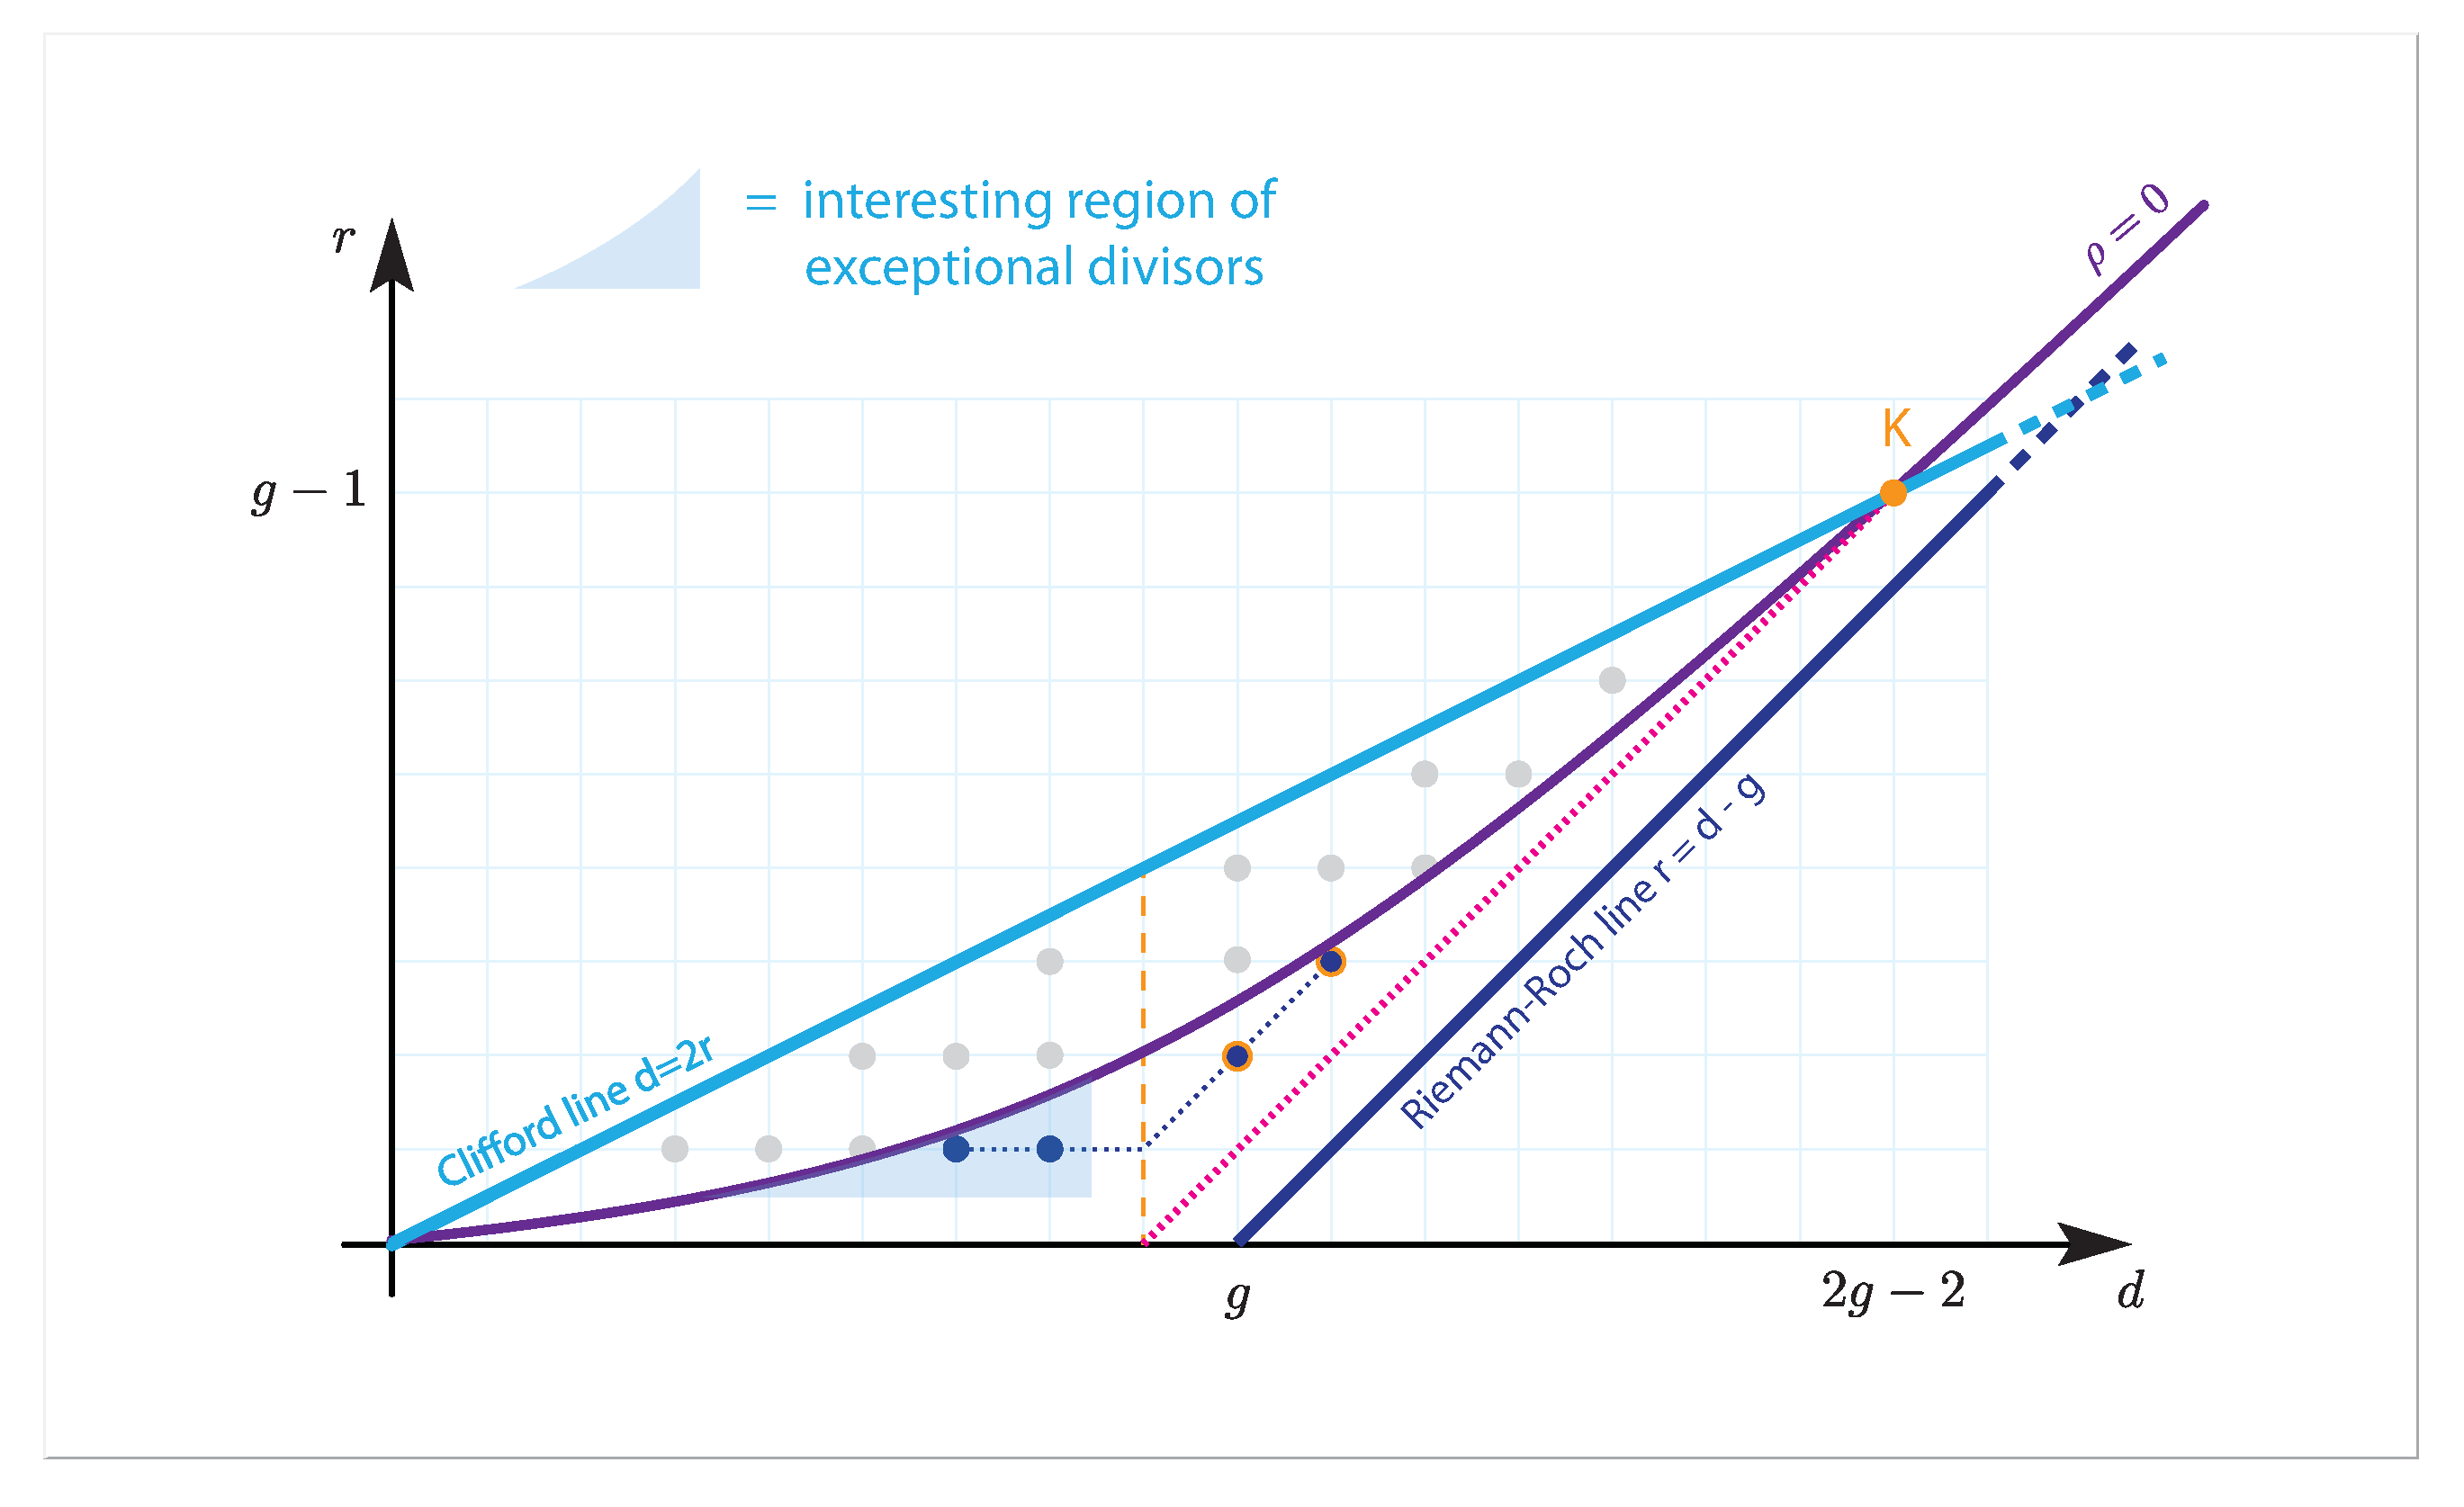
\includegraphics[width=\textwidth]{Exceptional_Divisors_BN.pdf}
		\caption{The interesting region of exceptional special divisors in the case of a curve of genus $g=9$, further refined exploiting the Dimension Theorem }
	\end{figure}








